% ****** Start of file apssamp.tex ******
%
%   This file is part of the APS files in the REVTeX 4.1 distribution.
%   Version 4.1r of REVTeX, August 2010
%
%   Copyright (c) 2009, 2010 The American Physical Society.
%
%   See the REVTeX 4 README file for restrictions and more information.
%
% TeX'ing this file requires that you have AMS-LaTeX 2.0 installed
% as well as the rest of the prerequisites for REVTeX 4.1
%
% See the REVTeX 4 README file
% It also requires running BibTeX. The commands are as follows:
%
%  1)  latex apssamp.tex
%  2)  bibtex apssamp
%  3)  latex apssamp.tex
%  4)  latex apssamp.tex
%
\documentclass[%
 reprint,
%superscriptaddress,
%groupedaddress,
%unsortedaddress,
%runinaddress,
%frontmatterverbose, 
%preprint,
%showpacs,preprintnumbers,
%nofootinbib,
%nobibnotes,
%bibnotes,
 amsmath,amssymb,
 aps,
%pra,
%prb,
%rmp,
%prstab,
%prstper,
%floatfix,
]{revtex4-1}

\usepackage{graphicx}% Include figure files
\graphicspath{{figures/}}
\usepackage{dcolumn}% Align table columns on decimal point
\usepackage{bm}% bold math
%\usepackage{hyperref}% add hypertext capabilities
%\usepackage[mathlines]{lineno}% Enable numbering of text and display math
%\linenumbers\relax % Commence numbering lines

%\usepackage[showframe,%Uncomment any one of the following lines to test 
%%scale=0.7, marginratio={1:1, 2:3}, ignoreall,% default settings
%%text={7in,10in},centering,
%%margin=1.5in,
%%total={6.5in,8.75in}, top=1.2in, left=0.9in, includefoot,
%%height=10in,a5paper,hmargin={3cm,0.8in},
%]{geometry}

\begin{document}

\preprint{APS/123-QED}

\title{Dissipative particle dynamics simulation of cell entry into a micro-channel}% Force line breaks with \\
%\thanks{A footnote to the article title}%

\author{Lvwen Zhou}
\affiliation{Institute of Mechanics, Chinese Academy of Sciences, Beijing 100190, China}
\author{Yu-Qian Zhang}
\affiliation{Cancer Institute \& Hosptial, Chinese Academy of Medical Sciences, Beijing 100021, China}
\author{Xiao-Long Deng}
\affiliation{Beijing Computational Science Research Center, Beijing 100084, China}
\author{Moubin Liu}
\email{mbliu@pku.edu.cn}
\affiliation{College of Engineering, Peking University, Beijing 100871, China}

 %\altaffiliation[Also at ]{Physics Department, XYZ University.}%Lines break automatically or can be forced with \\
%\author{Second Author}%
% \email{Second.Author@institution.edu}
%\affiliation{%
% Authors' institution and/or address\\
% This line break forced with \textbackslash\textbackslash
%}%

%\collaboration{MUSO Collaboration}%\noaffiliation

%\author{Charlie Author}
% \homepage{http://www.Second.institution.edu/~Charlie.Author}
%\affiliation{
% Second institution and/or address\\
% This line break forced% with \\
%}%
%\affiliation{
% Third institution, the second for Charlie Author
%}%
%\author{Delta Author}
%\affiliation{%
% Authors' institution and/or address\\
% This line break forced with \textbackslash\textbackslash
%}%

%\collaboration{CLEO Collaboration}%\noaffiliation

\date{\today}% It is always \today, today,
             %  but any date may be explicitly specified

\begin{abstract}
Cell deformability is an important biomarker which can be used to distinguish and sort between healthy and cancer cells. In this paper, we presented a dissipative particle dynamics (DPD) model for investigating cell entry into micro-channels. The cell membrane is represented by a network of DPD particles (beads) connected by worm-like chain (WLC) springs, which is able to mimic the viscoelastic effect of the membrane.  The entry process of benign breast epithelial cells (MCF-10A) and non-metastatic tumor breast cells (MCF-7) through a constricted micro-channel are comparatively investigated using this DPD model.  It is shown that both the time histories of the cell displacement and the dynamic behaviors of cell entry agree with experimental observations. The entry time of MCF-10A cell is approximately four times of that of MCF-7 cell since MCF-10A cells are stiffer than MCF-7 cells.  It is demonstrated that the presented DPD method is effective in modeling cell deformability, and the obtained results can be helpful in understanding how cells with different mechanical properties respond to physical loads.
%\begin{description}
%\item[Usage]
%Secondary publications and information retrieval purposes.
%\item[PACS numbers]
%May be entered using the \verb+\pacs{#1}+ command.
%\item[Structure]
%You may use the \texttt{description} environment to structure your abstract;
%use the optional argument of the \verb+\item+ command to give the category of each item. 
%\end{description}
\end{abstract}

\pacs{Valid PACS appear here}% PACS, the Physics and Astronomy
                             % Classification Scheme.
%\keywords{Suggested keywords}%Use showkeys class option if keyword
                              %display desired
\maketitle

%\tableofcontents

\section{Introduction}

Dynamical behaviors of migration and deformation variations of cells in confined environment are probably caused by pathological changes in mechanical properties of cells, which may be closely related to several cell diseases. These variations are often facilitated by the altering in the mechanical behaviors of cells such as large changes of elastic modulus \cite{hosseini_particle-based_2009}. Modern physiology and medicine have established the relationship of mechanical variations between healthy and pathological cells. For example, compared to healthy cells, diseased cells such as cancer cells are known to have different stiffness and elasticity \cite{lee_biomechanics_2007}. Such differences can be used to distinguish between normal and diseased cells \cite{bathe_neutrophil_2002,hou_deformability_2009}. Recently, increased micro-fluidic devices were designed and applied in medical diagnostics to diagnose and treat cells disease \cite{suresh_biomechanics_2007,liu_microfluidic_2010}. 
Thus, investigating cell entry into micro channels can be fundamentally important and it is of significance to understand how cells with different mechanical properties respond to physical loads, and to further design more effective micro-fluidic devices. 

In this work, we present a DPD model for simulating the entry process of  MCF-10A and MCF-7 cells through a constricted micro-channel. Cell model is described in section \ref{cell}.  Numerical simulations of MCF-10A and MCF-7 cells through a constricted micro-channel are presented and analyzed in section \ref{simulation} and \ref{results}. The paper concludes in section \ref{conclusion} with some remarks. 

%%%%%%%%%%%%%%%%%%%%%%%%%%%%%%%%%%%%%%%%%%%%%%%%%%%%%%%%%%%%%%%%%%%%%%%%%%%%%%

\section{Methods}\label{cell}

\subsection{DPD method}
Dissipative particle dynamics (DPD) \cite{hoogerbrugge_simulating_1992} is a mesoscopic method which describes clusters of molecules (particle) moving together in a Lagrangian fashion subject to soft quadratic potentials. The total force acting on a DPD particle $i$ is given by a sum over all particles $j$ that lie within a fixed cut-off distance, of three pairwise-additive forces:
\begin{equation}\label{Forcesum}
\mathbf{f}_{i}  = \sum_{j\neq i} \mathbf{F}_{ij}^\mathrm{C} + \mathbf{F}_{ij}^\mathrm{D} + \mathbf{F}_{ij}^\mathrm{R}
\end{equation}
where $\mathbf{F}_{ij}^\mathrm{C}$ is a conservative force, $\mathbf{F}_{ij}^\mathrm{D}$ and $\mathbf{F}_{ij}^\mathrm{R}$ is a dissipative force and a random force. The conservative force acts to give particle a chemical identity, while the dissipative and random forces together form a thermostat that keeps the mean temperature of the system constant. For more detailed information about methodology and applications of DPD, see Refs. \cite{hoogerbrugge_simulating_1992,liu_dissipative_2014}.

% ----------------------------------------------------------------------------

\subsection{Cell membrane model}
In this section, we construct cell membrane model using DPD. There are four types of particles in our DPD system,  as shown in Fig. \ref{fig:4particles}. The non-slip boundary condition is implemented by using frozen particles in the solid obstacle areas together with the Maxwellian reflection model when a fluid particle enters a thin reflecting boundary layer. This solid boundary treatment has been proven to be effective in preventing unphysical particle penetration and density oscillations can be controlled in a reasonably low level \cite{Liu_particle_2016,liu_dissipative_2014,liu_dissipative_2007,zhou_movement_2013}.
\begin{figure}[!htb]
\centering
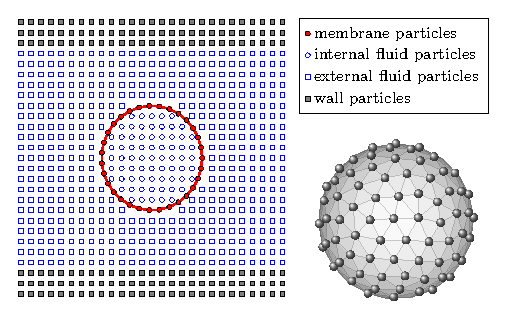
\includegraphics{4typeparticles.eps}
\caption{(Color online) DPD system with four types of particles. Cell membrane model is represented by a network of springs linked DPD particles.}\label{fig:4particles}
\end{figure}
The cell membrane structure is defined by a two-dimensional triangular network on the spherical surface. Each link of triangular network is modelled by nonlinear WLC spring model \cite{marko_stretching_1995}. The force between membrane particles includes the elastic and viscous parts. The elastic part is characterized by an energy potential, given by
\begin{equation}\label{eq:free_energy} 
U(\{\mathbf{r}_i\}) = U_{\textrm{in-plane}} + U_{\mathrm{bending}} + U_{\mathrm{volume}}
\end{equation}


\section{Simulation}\label{simulation}
In Hou et al.'s study \cite{hou_deformability_2009}, a microfabricated fluidic channel design consisting of a straight channel and two reservoirs, as shown in Fig. \ref{fig:experimental_setup}, was used to study the biorheological behaviour of MCF-10A cells and MCF-7 cells to develop a method to distinguish between non-malignant and malignant cells. 
The fluidic channel is 150 $\mu m$ in length and has a square cross section area of 10 by 10 $\mu m$ with a 45$^\circ$ tapered entrance. Flow in the micro-channel is driven by a differential pressure $\Delta p = 490.5 \mathrm{Pa}$ established between both ends of the setup. Under experimental conditions at room temperature of 22-24$^\circ\mathrm{C}$, the cells have to deform to pass through the channel, allowing quantification of several physical parameters such as entry time, transit velocity and elongation index. 
\begin{figure}[!htb]
\centering
\includegraphics{3Dchannel.eps}
\caption{Schematic of a micro-channel with a tapered entrance.}\label{fig:experimental_setup}
\end{figure}

In the present study, we numerically investigate the entry of MCF-10A cells and MCF-7 cells into a micro-channel by using method described in previous sections. The diameters of the cells are based on mean experimental values of $20 \pm 5 \mu m$, and in this paper it is taken to be $D^\mathrm{P} = 20 \mu m$. For MCF-7 cells, the Young's modulus is taken to be $Y^\mathrm{P} = 0.02\mathrm{dyn/cm}=2\times 10^{-5} \mathrm{N/m}$ referenced from the range of literature values (0.005-0.035$\mathrm{dyn/cm}$) \cite{leong_modeling_2011}. MCF-7 cells were found to have an apparent Young's modulus significantly lower (1.4-1.8 times) than that of their non-malignant (MCF-10A) counterparts \cite{li_afm_2008}. For MCF-10A cells, the Young's modulus is taken to be 1.6 times of their MCF-7 counterparts. The selected value of bending rigidity is $k_c = 6.93\times 10^{-20}\mathrm{J}$ referenced from the range of literature values (4-9$\times 10^{-20}\mathrm{J}$) \cite{evans_entropy-driven_1990}. Room temperature is taken to be $T^\mathrm{P} = 296.15\mathrm{K}$). It is not convenient for DPD simulation driven by a differential pressure as in the experiment, we use the following formula to translate differential pressure to a body force exerting on every DPD particle.
\begin{equation}
g^\mathrm{M} = \frac{\Delta P S^\mathrm{P}}{\rho^\mathrm{M} L^\mathrm{M} S^\mathrm{M}}\frac{1}{\zeta} 
= \frac{\Delta P \lambda^3}{\rho^\mathrm{M} L^\mathrm{P}}\frac{1}{\zeta} 
\end{equation}

%%%%%%%%%%%%%%%%%%%%%%%%%%%%%%%%%%%%%%%%%%%%%%%%%%%%%%%%%%%%%%%%%%%%%%%%%%%%%%

\section{Results}\label{results}
In this section, MCF-10A cell is firstly studied by the DPD model and compared with the experiment, and then MCF-7 cell is also studied and compared with simulation results of MCF-10A cell. 

\subsection{MCF-10A passing through a contracted micro-channel}
In DPD simulation, the cell is initially positioned at a distance of 25 from the channel entrance to give the cell initial transient period to reach steady velocity before entry. Fig. \ref{fig:Snapshots-DPD} shows snapshots of MCF-10A cell through the micro-channel.
\begin{figure}[!htb]
\centering
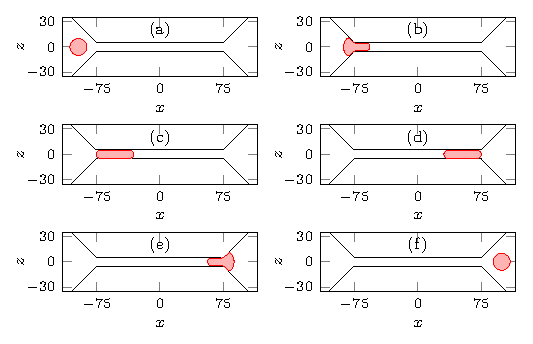
\includegraphics{Snapshots-DPD.eps}
\caption{(Color online) Snapshots of MCF-10A cell traversing across a micro-channel from DPD simulation at $t=0.00$s (a), $t=4.45$s (b), $t=16.41$s (c), $t=23.32$s (d), $t=24.92$s (e) and $t=29.79$s (f).} \label{fig:Snapshots-DPD}
\end{figure}


%%%%%%%%%%%%%%%%%%%%%%%%%%%%%%%%%%%%%%%%%%%%%%%%%%%%%%%%%%%%%%%%%%%%%%%%%%%%%%

\section{Conclusion}\label{conclusion}

This paper presented a DPD model for simulating the movement and deformability of single cells when entering micro-channels with confined structures.  The entry processes of MCF-10A and MCF-7 cells are comparatively investigated. We conclude that the presented DPD method with WLC spring to model cells is effective in simulating cell entry into micro-channels. Both the cell displacement time-plots and the dynamical behavior of the cell entry are shown to match quantitatively throughout the cell entry, subjected to experimental uncertainties and model assumptions. Furthermore, the model allowed us to confirm that MCF-10A cells have longer entry time than MCF-7 cells of similar sizes because MCF-10A cells are stiffer than MCF-7 cells. These quantitative agreements show the usefulness and effectiveness of our models in interpreting cellular experiments.


\begin{acknowledgments}
This work has been supported by the National Natural Science Foundation of China (31370953, 10942004 and 91230203).
\end{acknowledgments}

%\appendix

%\section{Appendixes}
% The \nocite command causes all entries in a bibliography to be printed out
% whether or not they are actually referenced in the text. This is appropriate
% for the sample file to show the different styles of references, but authors
% most likely will not want to use it.
%\nocite{*}

\bibliography{main.bib}% Produces the bibliography via BibTeX.

\end{document}

